\documentclass[tikz, margin=0.1cm]{standalone}

\usepackage{stix2}

\begin{document}
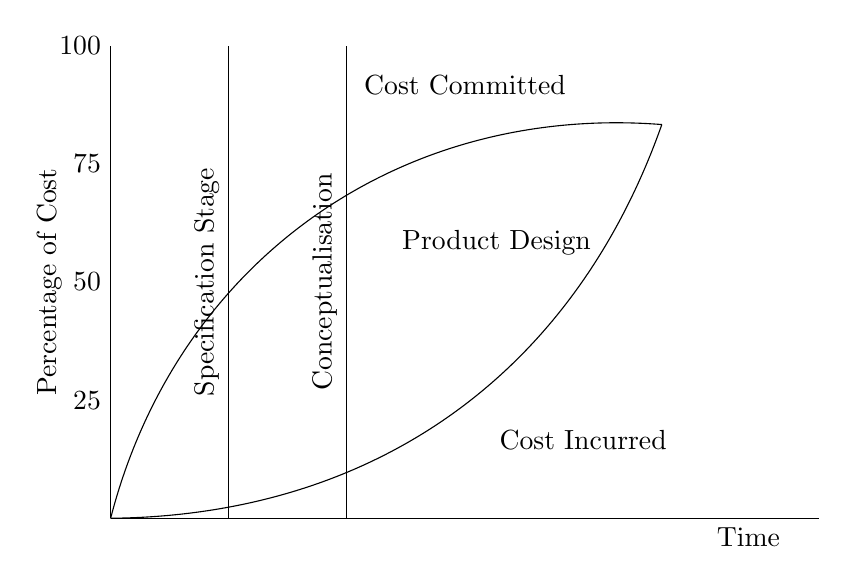
\begin{tikzpicture}

    \draw[] (0,0) -- (0,6)
        node[pos=0.25, anchor=east] {25}
        node[pos=0.50, anchor=east] {50}
        node[pos=0.75, anchor=east] {75}
        node[pos=1.00, anchor=east] {100}
        node[pos=0.50, rotate=90, anchor=south, yshift=0.5cm] {Percentage of Cost};
    \draw[] (0,0) -- (9,0)
        node[pos=0.9, anchor=north] {Time};
    
    %\draw[] plot [smooth] coordinates {(0,0) (4,1.5) (8,5)};
    \draw[] (0,0) to [bend right=35] (7,5);
    \draw[] (0,0) to [bend left=40] (7,5);
    
    \draw[] (1.5,0) -- (1.5,6) node[pos=0.5, anchor=south, rotate=90] {Specification Stage};
    \draw[] (3,0) -- (3,6) node[pos=0.5, anchor=south, rotate=90] {Conceptualisation};
    
    \node[] at (6,1) {Cost Incurred};
    \node[] at (4.9,3.5) {Product Design};
    \node[] at (4.5,5.5) {Cost Committed};
    
\end{tikzpicture}
\end{document}